\section{Fisher Exact Test}
Sir Ronald A. Fisher, the English statistician, has been called the
father of modern statistics.

\subsection{The Lady Tasting Tea}
A famous story, in Cambridge, England, in the late 1920is, that a colleague of Fisher's claimed that she
could tell, while drinking tea with milk, whether milk or tea was
poured into the cup first. 

An experiment was designed to test her claim.
\begin{itemize}
	\item 8 cups of tea were presented to her in a random order; 4 of these
	had milk poured first while the other 4 had tea poured first.
	\item She was told that there were 4 cups of each type.
\end{itemize}

Suppose we have the following data show the results of the experiment. 
\begin{figure}[H]
	\centering
	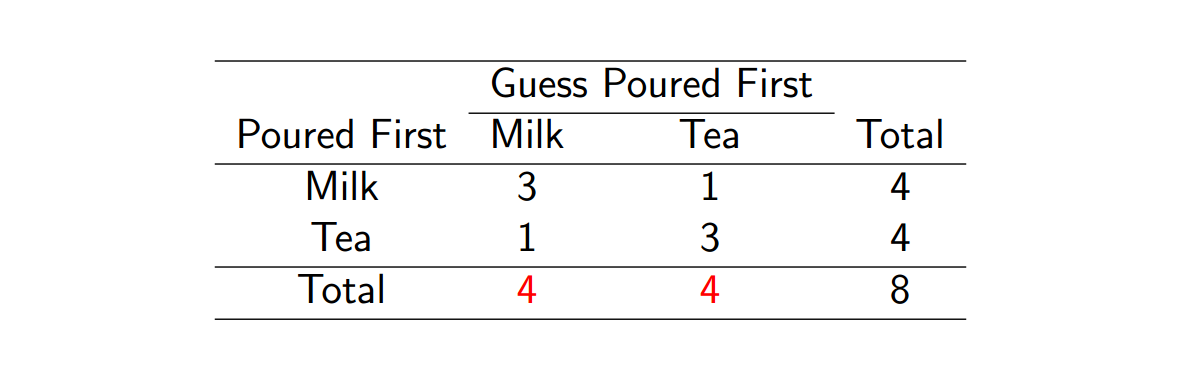
\includegraphics[width=0.7\linewidth]{fig/screenshot004}
	\caption{Contingenvy Table of Lady Tasting Tea}
	\label{fig:screenshot004}
\end{figure}

One can observe that she was right 3 out of 4 times on both types. Is this sufficient
evidence to support her claim of special power?

The contingency table has two difference comparing with the one we met.
\begin{itemize}
	\item The columns are fixed.
	\item The sample size is very small.
\end{itemize}

\subsection{Review: Hyper-geometric Distribution}
Suppose there are $m$ red balls and $n - m$ green balls. We randomly
pick $k$ balls without replacement. What is the probability that $z$ balls
are red?

Let $Z$ be the number of red balls.
\[\P(Z = z) = \frac{{m \choose z} {n-m \choose k - z}}{{n \choose k}}, z = 0, 1, \cdots, k.\]

Here we assume that
\begin{itemize}
	\item $z \le k$
	\item $z \le m$
	\item $k - z \le n - m$
\end{itemize}

\subsubsection{Example}

Suppose we have the following contingency table, in other words, $m = 6$, $n - m = 19$, $n = 25$. Also, $k = 10$ and $z = 1$. 
\begin{figure}[H]
	\centering
	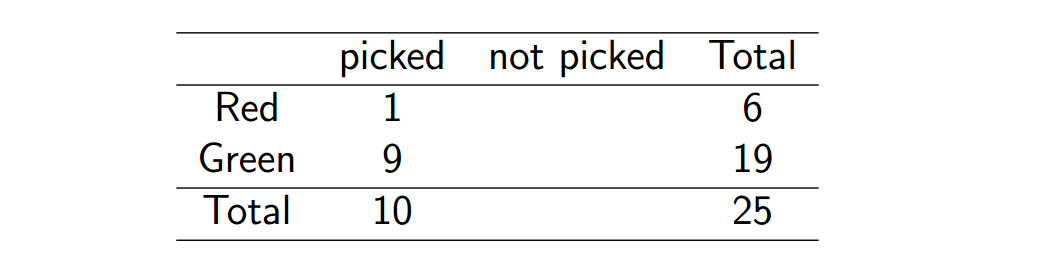
\includegraphics[width=0.7\linewidth]{fig/screenshot005}
	\caption{Hyper-geometric Distribution Example}
	\label{fig:screenshot005}
\end{figure}

We have
\[\P(Z = 1) = \frac{{6 \choose 1}{19 \choose 9}}{{25 \choose 10}}\]

The pdf of hyper-geometric distribution in R is as follows.
\begin{lstlisting}[language=R]
choose(6,1)*choose(19,9)/choose(25,10)
dhyper(x=1, m=6, 19, k=10)
\end{lstlisting}
\subsection{Fisher Exact Test}
Applying the hyper-geometric distribution, conditional on 4 guesses of having milk added first, the probability of
3 correct guesses is
\[\P(Z = 3) = \frac{{4 \choose 3}{4 \choose 4 - 3}}{{8 \choose 4}} = 0.229\]

So if the lady cannot tell the difference between two types of mix, there is still $22.9\%$ of probability for her to have 3 correct guesses by chance. Then how to exam her claim? Hypothesis Testing. To be more specific, Fisher Exact Test.

\subsection{Exact Inference for Small Samples}
The setup of Fisher Exact Test can be represented by the following contingency table.

\begin{figure}[H]
	\centering
	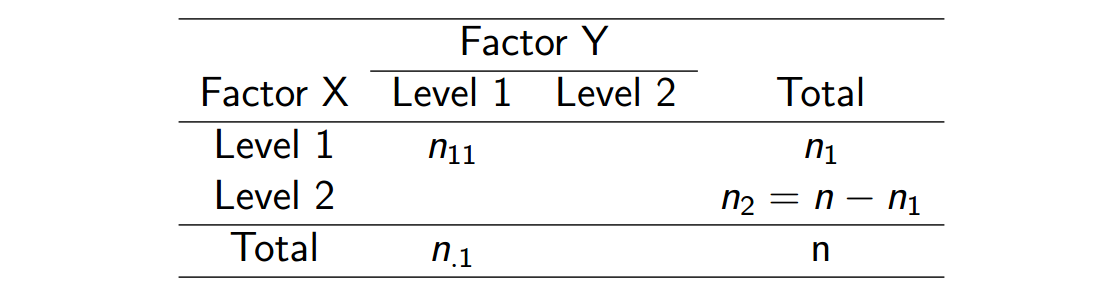
\includegraphics[width=0.7\linewidth]{fig/screenshot006}
	\caption{Contingency Table of Fisher Exact Test}
	\label{fig:screenshot006}
\end{figure}

In the table, $n_1$, $n$, and $n_{.1}$ are fixed. We can infer that $n_{.2} = n - n_{.1}$. $n_{11}$ is the observed random variable.

Fisher's exact test is based on the conditional distribution of $n_{11}$ given $n_1$, $n$, and $n_{.1}$. Given, $z \le \min\{n_1, n_{.1}\}$, and $n_{.1} - z \le n_2$,
\[\P(n_{11} = z) = \frac{{n_1 \choose z} {n_2 \choose n_{.1} - z}}{{n \choose n_{.1}}}.\]

Recall that the $p$-value is calculated by the sum of all event which are equal or rarer than the observed event.

Note that the estimated odd ratio is different from the calculation we have been using. It is because that the experiment design is different with the ones we have. The estimation of odd ratio can be found in R's fisher test manual.
\lstinputlisting[language=R]{code/l10-fisher-exact.R}
